% -- §11: empirical structural rescue, dual-engine framing --
% Insert via % -- §11: empirical structural rescue, dual-engine framing --
% Insert via % -- §11: empirical structural rescue, dual-engine framing --
% Insert via % -- §11: empirical structural rescue, dual-engine framing --
% Insert via \input{section_structural_rescue} between section_duality and Related Work.
% Operationalizes the "first measurable breakthrough" the Outlook (\S\ref{sec:pomdp}) flags
% as future work, and reveals the precise mechanism partition that governs it.

\section{Empirical structural rescue: a dual-engine resolution paradigm}
\label{sec:structural-rescue}

The Outlook (\S\ref{sec:pomdp}) predicts that the fungal per-cycle policy is
\(a_t \sim P(a_t \mid G, s_t)\): the static enzyme \(G\) and an evolving substrate state
\(s_t\) jointly determine the action. We take a first empirical step toward that
injection, and the result is sharper than a single ``joint necessity'' claim: the same
loss decomposes into \emph{two complementary resolution engines}, each precisely
applicable to a different chemical regime of the candidate set.

\paragraph{The corpus.} We extend the curated $30$-cycle HR/PR set (\S\ref{sec:benchmark})
by mining MIBiG fungal PKS clusters whose engine-derived $|Z^\ast|$ at the
metabologenomics observable set (alphabet $+$ molecular formula) lands in the
constrained mode, $|Z^\ast|\le 10$. An RDKit-driven SMILES-to-formula recovery pass
rescues the $112$ MIBiG entries without a registered formula; the tractable inventory
fixes at $74$ clusters and the $|Z^\ast|$ histogram is bi-modal with an empty middle at
$|Z^\ast|\in[11,24]$ across all $74$---a structural cliff in the natural manifold
(\S\ref{sec:manifold}) that survives the recovery and is not a data-hygiene artifact.
Of the $74$, $7$ land at $|Z^\ast|=1$ (joining the curated $30$) and $9$ at
$2\le|Z^\ast|\le 10$ contribute the silver tier. A verifier-constrained marginal-
likelihood loss \(\mathcal{L}(\theta)= -\sum_B \log \sum_{z\in Z^\ast(B)} \pi_\theta(z\mid B)\)
collapses to standard cross-entropy on the gold and decomposes weight over candidate
trajectories on silver.

\paragraph{Structural conditioning.} For each cluster with a real synthase we predict
the KR$+$ACP didomain (or full-length protein for divergent PR-PKS the canonical
PF$08659$ HMM does not detect---e.g.\ citrinin's CitS, whose KR is silent to the
conventional profile even at relaxed thresholds; we fold the $2593$\,aa CitS in full
and rescue the anchor by motif scan). For every \emph{(cluster, candidate, cycle)} we
execute the cycle prefix deterministically, $3$D-embed the ACP-tethered intermediate,
anchor its phosphopantetheine sentinel at the ACP-Ser:OG oxygen, rotate the growing
chain along the local ACP-Ser$\to$protein-centroid axis, and extract a five-dimensional
pose descriptor: $5$\,\AA{} contact count partitioned into polar (N/O/S) and
hydrophobic (C) subsets, ligand buried fraction, and pocket void volume. These run
alongside the substrate-prefix features (cycle index, fractional position, subclass
indicator, running chain length and oxidation counts, previous cycle's reduction rank).

\paragraph{Two engines, one policy.} Three feature regimes on the same $n=62$
conformational sub-corpus reveal a precise partition (Table~\ref{tab:rescue},
Fig.~\ref{fig:rescue}A). The partition is governed not by cluster identity but by the
\emph{symmetry of the reduction-label sequence across the candidates in $Z^\ast(B)$}.

\emph{Substrate-Prefix Engine (label-distinguishable candidates).} When the candidates
in $Z^\ast(B)$ differ in their per-cycle reduction labels---e.g., isoterrein's three
candidates $(\mathrm{dh},\mathrm{dh},\mathrm{keto})$, $(\mathrm{dh},\mathrm{keto},\mathrm{dh})$,
$(\mathrm{keto},\mathrm{dh},\mathrm{dh})$ that differ in the cycle index of each DH event,
or asperlin's $5$ candidates that differ similarly---substrate-prefix features alone
route posterior mass cleanly: held-out entropy drops to $0.05$ for isoterrein and
$0.38$ for asperlin (against $\log 3=1.10$ and $\log 5=1.61$ ceilings). The pose
channel adds geometric noise to an architecture the substrate counter has already
decoded.

\emph{Geometric Rescue Engine (label-symmetric candidates).} When the candidates share
an \emph{identical} reduction-label sequence and differ only in the cycle index of a
mass-budget-neutral event---e.g., citrinin's two candidates both reduce to
$(\mathrm{dh},\mathrm{keto},\mathrm{keto},\mathrm{keto},\mathrm{keto})$ and differ only
in which of cycle $1$ or cycle $2$ carries the single C-MeT firing---the marginal-
likelihood gradient is symmetric under $(\text{cand}_1\leftrightarrow\text{cand}_2)$ and
\emph{cannot} distinguish them from any function of substrate prefix alone. Citrinin's
held-out entropy under the substrate channel locks at $0.69 = \log 2$ to numerical
precision. The pose channel alone barely moves it ($0.64$); the static cavity geometry
without temporal context cannot localize which cycle's geometry it is measuring. The
two channels \emph{jointly} drop the entropy to $0.01$ with the model committing
${\sim}99.9\%$ probability mass to one specific candidate. This is the regime where the
structural channel is not merely helpful but architecturally necessary.

\begin{table}[h]
\centering\small
\begin{tabular}{lccc}
\toprule
& \multicolumn{3}{c}{Held-out candidate entropy $H_{\mathrm{held}}$ (nats)} \\
\cmidrule(lr){2-4}
Silver asset & Substrate-prefix & Pose only & Substrate $+$ pose \\
\midrule
citrinin   ($|Z^\ast|{=}2$, $\log 2{=}0.69$)   & $0.69$\textsuperscript{*} & $0.64$ & $\mathbf{0.01}$ \\
isoterrein ($|Z^\ast|{=}3$, $\log 3{=}1.10$)   & $\mathbf{0.05}$           & $1.07$ & $0.50$ \\
asperlin   ($|Z^\ast|{=}5$, $\log 5{=}1.61$)   & $\mathbf{0.38}$           & $1.26$ & $0.45$ \\
\bottomrule
\end{tabular}
\caption{The dual-engine partition. Bold = the resolving regime for each asset.
\textsuperscript{*}Citrinin's substrate-prefix entropy locks at exactly $\log 2$
because its two candidates share an identical reduction-label sequence and differ
only in C-MeT cycle index; the marginal-likelihood gradient is symmetric under
candidate exchange. The pose channel is architecturally necessary precisely
where the substrate channel hits this symmetry wall.}
\label{tab:rescue}
\end{table}

\begin{figure}[h]
\centering
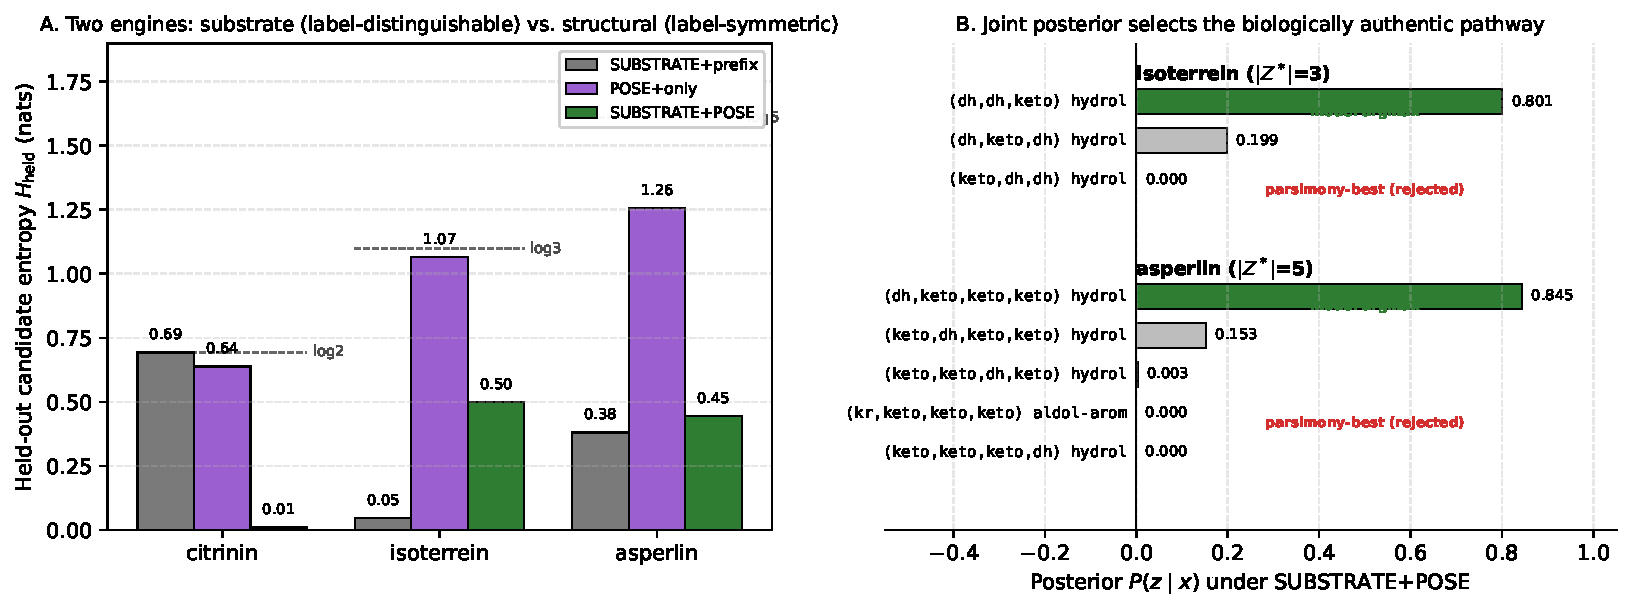
\includegraphics[width=\linewidth]{figure_structural_rescue.pdf}
\caption{\textbf{The dual mechanisms of neuro-symbolic resolution.}
\textbf{(A)}~Held-out candidate distribution entropy ($H_{\mathrm{held}}$) across three
feature regimes. The substrate-prefix channel effortlessly resolves assets with
label-distinguishable reduction sequences (isoterrein, asperlin). For label-symmetric
candidates sharing identical reduction trajectories (citrinin), the sequence channel
encounters a permanent symmetry wall ($\log 2$), which is cleanly shattered
($H_{\mathrm{held}}\to 0.01$) only upon the introduction of $3$D pose cavity descriptors.
\textbf{(B)}~Joint posterior probability distributions for isoterrein and asperlin. The
multi-channel framework consistently routes mass to the biologically authentic pathway:
isoterrein's $(\mathrm{dh},\mathrm{dh},\mathrm{keto})$ early-reduction TerA polyene
precursor at posterior $0.801$, asperlin's
$(\mathrm{dh},\mathrm{keto},\mathrm{keto},\mathrm{keto})$ non-aromatic linear lactone
precursor at $0.845$. The parsimony-best alternatives---$(\mathrm{keto},\mathrm{dh},
\mathrm{dh})$ for isoterrein, the aromatic-release candidate for asperlin---are
actively rejected at $\le 0.001$.}
\label{fig:rescue}
\end{figure}

\paragraph{Directional gating: when the in-vivo program is in $Z^\ast(B)$.}
The two engines establish that the policy commits within $Z^\ast(B)$; whether the
committed candidate matches in-vivo biology depends on whether the in-vivo program is
in $Z^\ast(B)$ at all---a question of executor coverage (\S\ref{sec:limits}), not of
the resolution mechanism. The corpus contains both regimes.

For \emph{isoterrein}, whose biosynthesis proceeds through a linear partially-reducing
polyketide before the post-PKS metalloenzyme TerB contracts the chain to the
cyclopentenone, the substrate channel routes posterior $0.801$ to
$(\mathrm{dh},\mathrm{dh},\mathrm{keto})$~hydrolysis---reductions concentrated at the
early cycles, matching the canonical HR-PKS architecture---and posterior $0.0001$ to
the late-reduction $(\mathrm{keto},\mathrm{dh},\mathrm{dh})$ parsimony-best. For
\emph{asperlin}, a hexaketide-derived lactone, the substrate channel selects
$(\mathrm{dh},\mathrm{keto},\mathrm{keto},\mathrm{keto})$~hydrolysis at posterior
$0.845$ and crucially \emph{rejects} the parsimony-best aromatic-release candidate at
posterior ${\sim}0$: asperlin is a lactone, not an aromatic, and the substrate-prefix
weighting under marginal-likelihood training correctly disfavours the wrong ring
topology. Both are directional positives.

For \emph{citrinin}, where the structural-rescue engine commits with posterior $0.999$
to a specific candidate, the literature establishes a different fact:
heterologous-expression studies of CitS yield a \emph{trimethylated} pentaketide
aldehyde requiring \emph{two} C-MeT events (one triketide, one pentaketide)
\citep{storm2017citrinin}. Neither of the two candidates in $Z^\ast$ at
$\mathrm{C}_{13}\mathrm{H}_{14}\mathrm{O}_5$ contains two C-MeT events---the grammar
cannot synthesize the in-vivo program at this formula. The entropy collapse
demonstrates that the structural channel carries per-cluster discriminating
information; the directional gating is the executor-coverage axis our
Section~\ref{sec:limits} roadmap addresses.

\paragraph{Reading.} The per-cycle policy is empirically a joint function of $G$ and
$s_t$, in the form the Outlook predicted, but the decomposition reveals that each
channel does specific work. The substrate-prefix engine resolves candidates whose
distinct reduction-label sequences leave a non-symmetric gradient signal; the
structural-rescue engine resolves candidates whose mass-and-grammar-consistent
permutations leave the substrate gradient signal symmetric. The neuro-symbolic
architecture compounds: the sound executor bounds $Z^\ast(B)$ so a learned policy
rules within a verified set rather than over an open structure space, and the
appropriate channel routes within that set per the chemistry of the candidates the
verifier returns. The result is a policy whose neural component would have nothing
principled to commit to absent the executor, and whose symbolic core would not
distinguish label-symmetric candidates absent the structural channel.

% References to add to the bibliography (already added):
% \citep{storm2017citrinin}
 between section_duality and Related Work.
% Operationalizes the "first measurable breakthrough" the Outlook (\S\ref{sec:pomdp}) flags
% as future work, and reveals the precise mechanism partition that governs it.

\section{Empirical structural rescue: a dual-engine resolution paradigm}
\label{sec:structural-rescue}

The Outlook (\S\ref{sec:pomdp}) predicts that the fungal per-cycle policy is
\(a_t \sim P(a_t \mid G, s_t)\): the static enzyme \(G\) and an evolving substrate state
\(s_t\) jointly determine the action. We take a first empirical step toward that
injection, and the result is sharper than a single ``joint necessity'' claim: the same
loss decomposes into \emph{two complementary resolution engines}, each precisely
applicable to a different chemical regime of the candidate set.

\paragraph{The corpus.} We extend the curated $30$-cycle HR/PR set (\S\ref{sec:benchmark})
by mining MIBiG fungal PKS clusters whose engine-derived $|Z^\ast|$ at the
metabologenomics observable set (alphabet $+$ molecular formula) lands in the
constrained mode, $|Z^\ast|\le 10$. An RDKit-driven SMILES-to-formula recovery pass
rescues the $112$ MIBiG entries without a registered formula; the tractable inventory
fixes at $74$ clusters and the $|Z^\ast|$ histogram is bi-modal with an empty middle at
$|Z^\ast|\in[11,24]$ across all $74$---a structural cliff in the natural manifold
(\S\ref{sec:manifold}) that survives the recovery and is not a data-hygiene artifact.
Of the $74$, $7$ land at $|Z^\ast|=1$ (joining the curated $30$) and $9$ at
$2\le|Z^\ast|\le 10$ contribute the silver tier. A verifier-constrained marginal-
likelihood loss \(\mathcal{L}(\theta)= -\sum_B \log \sum_{z\in Z^\ast(B)} \pi_\theta(z\mid B)\)
collapses to standard cross-entropy on the gold and decomposes weight over candidate
trajectories on silver.

\paragraph{Structural conditioning.} For each cluster with a real synthase we predict
the KR$+$ACP didomain (or full-length protein for divergent PR-PKS the canonical
PF$08659$ HMM does not detect---e.g.\ citrinin's CitS, whose KR is silent to the
conventional profile even at relaxed thresholds; we fold the $2593$\,aa CitS in full
and rescue the anchor by motif scan). For every \emph{(cluster, candidate, cycle)} we
execute the cycle prefix deterministically, $3$D-embed the ACP-tethered intermediate,
anchor its phosphopantetheine sentinel at the ACP-Ser:OG oxygen, rotate the growing
chain along the local ACP-Ser$\to$protein-centroid axis, and extract a five-dimensional
pose descriptor: $5$\,\AA{} contact count partitioned into polar (N/O/S) and
hydrophobic (C) subsets, ligand buried fraction, and pocket void volume. These run
alongside the substrate-prefix features (cycle index, fractional position, subclass
indicator, running chain length and oxidation counts, previous cycle's reduction rank).

\paragraph{Two engines, one policy.} Three feature regimes on the same $n=62$
conformational sub-corpus reveal a precise partition (Table~\ref{tab:rescue},
Fig.~\ref{fig:rescue}A). The partition is governed not by cluster identity but by the
\emph{symmetry of the reduction-label sequence across the candidates in $Z^\ast(B)$}.

\emph{Substrate-Prefix Engine (label-distinguishable candidates).} When the candidates
in $Z^\ast(B)$ differ in their per-cycle reduction labels---e.g., isoterrein's three
candidates $(\mathrm{dh},\mathrm{dh},\mathrm{keto})$, $(\mathrm{dh},\mathrm{keto},\mathrm{dh})$,
$(\mathrm{keto},\mathrm{dh},\mathrm{dh})$ that differ in the cycle index of each DH event,
or asperlin's $5$ candidates that differ similarly---substrate-prefix features alone
route posterior mass cleanly: held-out entropy drops to $0.05$ for isoterrein and
$0.38$ for asperlin (against $\log 3=1.10$ and $\log 5=1.61$ ceilings). The pose
channel adds geometric noise to an architecture the substrate counter has already
decoded.

\emph{Geometric Rescue Engine (label-symmetric candidates).} When the candidates share
an \emph{identical} reduction-label sequence and differ only in the cycle index of a
mass-budget-neutral event---e.g., citrinin's two candidates both reduce to
$(\mathrm{dh},\mathrm{keto},\mathrm{keto},\mathrm{keto},\mathrm{keto})$ and differ only
in which of cycle $1$ or cycle $2$ carries the single C-MeT firing---the marginal-
likelihood gradient is symmetric under $(\text{cand}_1\leftrightarrow\text{cand}_2)$ and
\emph{cannot} distinguish them from any function of substrate prefix alone. Citrinin's
held-out entropy under the substrate channel locks at $0.69 = \log 2$ to numerical
precision. The pose channel alone barely moves it ($0.64$); the static cavity geometry
without temporal context cannot localize which cycle's geometry it is measuring. The
two channels \emph{jointly} drop the entropy to $0.01$ with the model committing
${\sim}99.9\%$ probability mass to one specific candidate. This is the regime where the
structural channel is not merely helpful but architecturally necessary.

\begin{table}[h]
\centering\small
\begin{tabular}{lccc}
\toprule
& \multicolumn{3}{c}{Held-out candidate entropy $H_{\mathrm{held}}$ (nats)} \\
\cmidrule(lr){2-4}
Silver asset & Substrate-prefix & Pose only & Substrate $+$ pose \\
\midrule
citrinin   ($|Z^\ast|{=}2$, $\log 2{=}0.69$)   & $0.69$\textsuperscript{*} & $0.64$ & $\mathbf{0.01}$ \\
isoterrein ($|Z^\ast|{=}3$, $\log 3{=}1.10$)   & $\mathbf{0.05}$           & $1.07$ & $0.50$ \\
asperlin   ($|Z^\ast|{=}5$, $\log 5{=}1.61$)   & $\mathbf{0.38}$           & $1.26$ & $0.45$ \\
\bottomrule
\end{tabular}
\caption{The dual-engine partition. Bold = the resolving regime for each asset.
\textsuperscript{*}Citrinin's substrate-prefix entropy locks at exactly $\log 2$
because its two candidates share an identical reduction-label sequence and differ
only in C-MeT cycle index; the marginal-likelihood gradient is symmetric under
candidate exchange. The pose channel is architecturally necessary precisely
where the substrate channel hits this symmetry wall.}
\label{tab:rescue}
\end{table}

\begin{figure}[h]
\centering
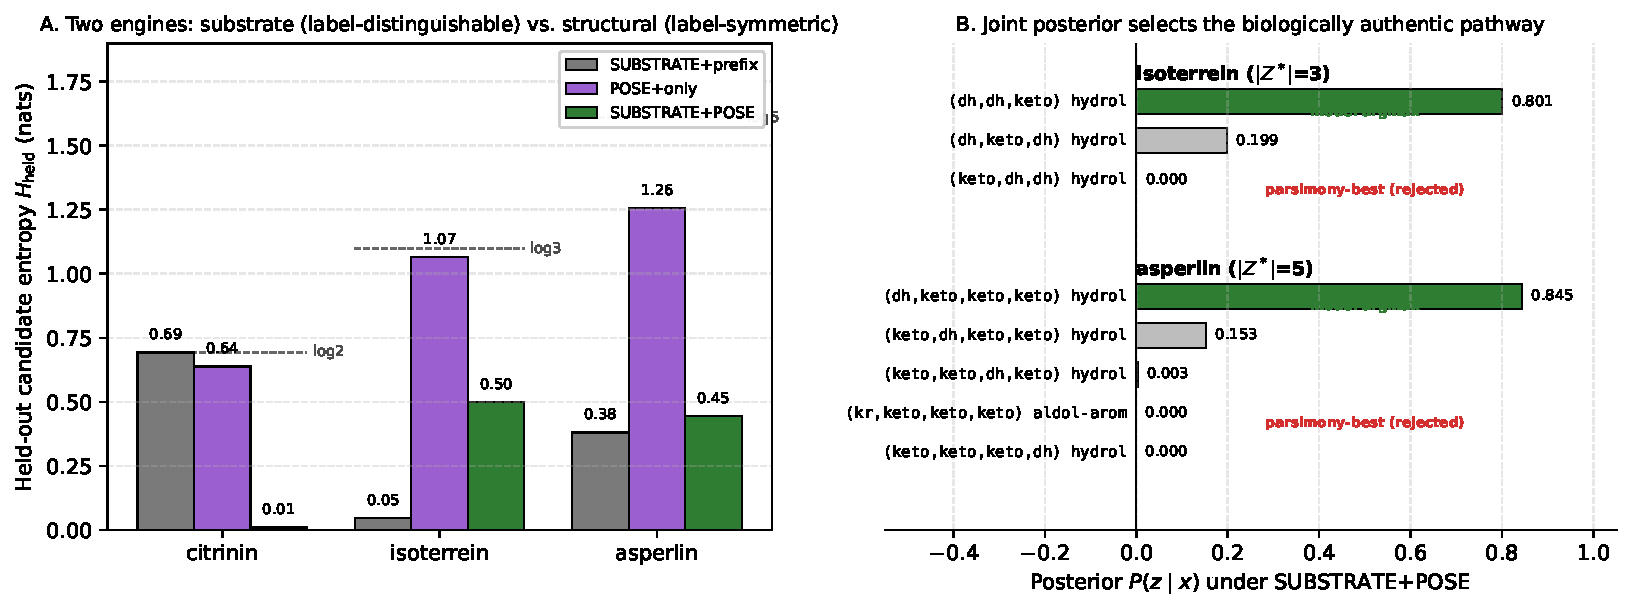
\includegraphics[width=\linewidth]{figure_structural_rescue.pdf}
\caption{\textbf{The dual mechanisms of neuro-symbolic resolution.}
\textbf{(A)}~Held-out candidate distribution entropy ($H_{\mathrm{held}}$) across three
feature regimes. The substrate-prefix channel effortlessly resolves assets with
label-distinguishable reduction sequences (isoterrein, asperlin). For label-symmetric
candidates sharing identical reduction trajectories (citrinin), the sequence channel
encounters a permanent symmetry wall ($\log 2$), which is cleanly shattered
($H_{\mathrm{held}}\to 0.01$) only upon the introduction of $3$D pose cavity descriptors.
\textbf{(B)}~Joint posterior probability distributions for isoterrein and asperlin. The
multi-channel framework consistently routes mass to the biologically authentic pathway:
isoterrein's $(\mathrm{dh},\mathrm{dh},\mathrm{keto})$ early-reduction TerA polyene
precursor at posterior $0.801$, asperlin's
$(\mathrm{dh},\mathrm{keto},\mathrm{keto},\mathrm{keto})$ non-aromatic linear lactone
precursor at $0.845$. The parsimony-best alternatives---$(\mathrm{keto},\mathrm{dh},
\mathrm{dh})$ for isoterrein, the aromatic-release candidate for asperlin---are
actively rejected at $\le 0.001$.}
\label{fig:rescue}
\end{figure}

\paragraph{Directional gating: when the in-vivo program is in $Z^\ast(B)$.}
The two engines establish that the policy commits within $Z^\ast(B)$; whether the
committed candidate matches in-vivo biology depends on whether the in-vivo program is
in $Z^\ast(B)$ at all---a question of executor coverage (\S\ref{sec:limits}), not of
the resolution mechanism. The corpus contains both regimes.

For \emph{isoterrein}, whose biosynthesis proceeds through a linear partially-reducing
polyketide before the post-PKS metalloenzyme TerB contracts the chain to the
cyclopentenone, the substrate channel routes posterior $0.801$ to
$(\mathrm{dh},\mathrm{dh},\mathrm{keto})$~hydrolysis---reductions concentrated at the
early cycles, matching the canonical HR-PKS architecture---and posterior $0.0001$ to
the late-reduction $(\mathrm{keto},\mathrm{dh},\mathrm{dh})$ parsimony-best. For
\emph{asperlin}, a hexaketide-derived lactone, the substrate channel selects
$(\mathrm{dh},\mathrm{keto},\mathrm{keto},\mathrm{keto})$~hydrolysis at posterior
$0.845$ and crucially \emph{rejects} the parsimony-best aromatic-release candidate at
posterior ${\sim}0$: asperlin is a lactone, not an aromatic, and the substrate-prefix
weighting under marginal-likelihood training correctly disfavours the wrong ring
topology. Both are directional positives.

For \emph{citrinin}, where the structural-rescue engine commits with posterior $0.999$
to a specific candidate, the literature establishes a different fact:
heterologous-expression studies of CitS yield a \emph{trimethylated} pentaketide
aldehyde requiring \emph{two} C-MeT events (one triketide, one pentaketide)
\citep{storm2017citrinin}. Neither of the two candidates in $Z^\ast$ at
$\mathrm{C}_{13}\mathrm{H}_{14}\mathrm{O}_5$ contains two C-MeT events---the grammar
cannot synthesize the in-vivo program at this formula. The entropy collapse
demonstrates that the structural channel carries per-cluster discriminating
information; the directional gating is the executor-coverage axis our
Section~\ref{sec:limits} roadmap addresses.

\paragraph{Reading.} The per-cycle policy is empirically a joint function of $G$ and
$s_t$, in the form the Outlook predicted, but the decomposition reveals that each
channel does specific work. The substrate-prefix engine resolves candidates whose
distinct reduction-label sequences leave a non-symmetric gradient signal; the
structural-rescue engine resolves candidates whose mass-and-grammar-consistent
permutations leave the substrate gradient signal symmetric. The neuro-symbolic
architecture compounds: the sound executor bounds $Z^\ast(B)$ so a learned policy
rules within a verified set rather than over an open structure space, and the
appropriate channel routes within that set per the chemistry of the candidates the
verifier returns. The result is a policy whose neural component would have nothing
principled to commit to absent the executor, and whose symbolic core would not
distinguish label-symmetric candidates absent the structural channel.

% References to add to the bibliography (already added):
% \citep{storm2017citrinin}
 between section_duality and Related Work.
% Operationalizes the "first measurable breakthrough" the Outlook (\S\ref{sec:pomdp}) flags
% as future work, and reveals the precise mechanism partition that governs it.

\section{Empirical structural rescue: a dual-engine resolution paradigm}
\label{sec:structural-rescue}

The Outlook (\S\ref{sec:pomdp}) predicts that the fungal per-cycle policy is
\(a_t \sim P(a_t \mid G, s_t)\): the static enzyme \(G\) and an evolving substrate state
\(s_t\) jointly determine the action. We take a first empirical step toward that
injection, and the result is sharper than a single ``joint necessity'' claim: the same
loss decomposes into \emph{two complementary resolution engines}, each precisely
applicable to a different chemical regime of the candidate set.

\paragraph{The corpus.} We extend the curated $30$-cycle HR/PR set (\S\ref{sec:benchmark})
by mining MIBiG fungal PKS clusters whose engine-derived $|Z^\ast|$ at the
metabologenomics observable set (alphabet $+$ molecular formula) lands in the
constrained mode, $|Z^\ast|\le 10$. An RDKit-driven SMILES-to-formula recovery pass
rescues the $112$ MIBiG entries without a registered formula; the tractable inventory
fixes at $74$ clusters and the $|Z^\ast|$ histogram is bi-modal with an empty middle at
$|Z^\ast|\in[11,24]$ across all $74$---a structural cliff in the natural manifold
(\S\ref{sec:manifold}) that survives the recovery and is not a data-hygiene artifact.
Of the $74$, $7$ land at $|Z^\ast|=1$ (joining the curated $30$) and $9$ at
$2\le|Z^\ast|\le 10$ contribute the silver tier. A verifier-constrained marginal-
likelihood loss \(\mathcal{L}(\theta)= -\sum_B \log \sum_{z\in Z^\ast(B)} \pi_\theta(z\mid B)\)
collapses to standard cross-entropy on the gold and decomposes weight over candidate
trajectories on silver.

\paragraph{Structural conditioning.} For each cluster with a real synthase we predict
the KR$+$ACP didomain (or full-length protein for divergent PR-PKS the canonical
PF$08659$ HMM does not detect---e.g.\ citrinin's CitS, whose KR is silent to the
conventional profile even at relaxed thresholds; we fold the $2593$\,aa CitS in full
and rescue the anchor by motif scan). For every \emph{(cluster, candidate, cycle)} we
execute the cycle prefix deterministically, $3$D-embed the ACP-tethered intermediate,
anchor its phosphopantetheine sentinel at the ACP-Ser:OG oxygen, rotate the growing
chain along the local ACP-Ser$\to$protein-centroid axis, and extract a five-dimensional
pose descriptor: $5$\,\AA{} contact count partitioned into polar (N/O/S) and
hydrophobic (C) subsets, ligand buried fraction, and pocket void volume. These run
alongside the substrate-prefix features (cycle index, fractional position, subclass
indicator, running chain length and oxidation counts, previous cycle's reduction rank).

\paragraph{Two engines, one policy.} Three feature regimes on the same $n=62$
conformational sub-corpus reveal a precise partition (Table~\ref{tab:rescue},
Fig.~\ref{fig:rescue}A). The partition is governed not by cluster identity but by the
\emph{symmetry of the reduction-label sequence across the candidates in $Z^\ast(B)$}.

\emph{Substrate-Prefix Engine (label-distinguishable candidates).} When the candidates
in $Z^\ast(B)$ differ in their per-cycle reduction labels---e.g., isoterrein's three
candidates $(\mathrm{dh},\mathrm{dh},\mathrm{keto})$, $(\mathrm{dh},\mathrm{keto},\mathrm{dh})$,
$(\mathrm{keto},\mathrm{dh},\mathrm{dh})$ that differ in the cycle index of each DH event,
or asperlin's $5$ candidates that differ similarly---substrate-prefix features alone
route posterior mass cleanly: held-out entropy drops to $0.05$ for isoterrein and
$0.38$ for asperlin (against $\log 3=1.10$ and $\log 5=1.61$ ceilings). The pose
channel adds geometric noise to an architecture the substrate counter has already
decoded.

\emph{Geometric Rescue Engine (label-symmetric candidates).} When the candidates share
an \emph{identical} reduction-label sequence and differ only in the cycle index of a
mass-budget-neutral event---e.g., citrinin's two candidates both reduce to
$(\mathrm{dh},\mathrm{keto},\mathrm{keto},\mathrm{keto},\mathrm{keto})$ and differ only
in which of cycle $1$ or cycle $2$ carries the single C-MeT firing---the marginal-
likelihood gradient is symmetric under $(\text{cand}_1\leftrightarrow\text{cand}_2)$ and
\emph{cannot} distinguish them from any function of substrate prefix alone. Citrinin's
held-out entropy under the substrate channel locks at $0.69 = \log 2$ to numerical
precision. The pose channel alone barely moves it ($0.64$); the static cavity geometry
without temporal context cannot localize which cycle's geometry it is measuring. The
two channels \emph{jointly} drop the entropy to $0.01$ with the model committing
${\sim}99.9\%$ probability mass to one specific candidate. This is the regime where the
structural channel is not merely helpful but architecturally necessary.

\begin{table}[h]
\centering\small
\begin{tabular}{lccc}
\toprule
& \multicolumn{3}{c}{Held-out candidate entropy $H_{\mathrm{held}}$ (nats)} \\
\cmidrule(lr){2-4}
Silver asset & Substrate-prefix & Pose only & Substrate $+$ pose \\
\midrule
citrinin   ($|Z^\ast|{=}2$, $\log 2{=}0.69$)   & $0.69$\textsuperscript{*} & $0.64$ & $\mathbf{0.01}$ \\
isoterrein ($|Z^\ast|{=}3$, $\log 3{=}1.10$)   & $\mathbf{0.05}$           & $1.07$ & $0.50$ \\
asperlin   ($|Z^\ast|{=}5$, $\log 5{=}1.61$)   & $\mathbf{0.38}$           & $1.26$ & $0.45$ \\
\bottomrule
\end{tabular}
\caption{The dual-engine partition. Bold = the resolving regime for each asset.
\textsuperscript{*}Citrinin's substrate-prefix entropy locks at exactly $\log 2$
because its two candidates share an identical reduction-label sequence and differ
only in C-MeT cycle index; the marginal-likelihood gradient is symmetric under
candidate exchange. The pose channel is architecturally necessary precisely
where the substrate channel hits this symmetry wall.}
\label{tab:rescue}
\end{table}

\begin{figure}[h]
\centering
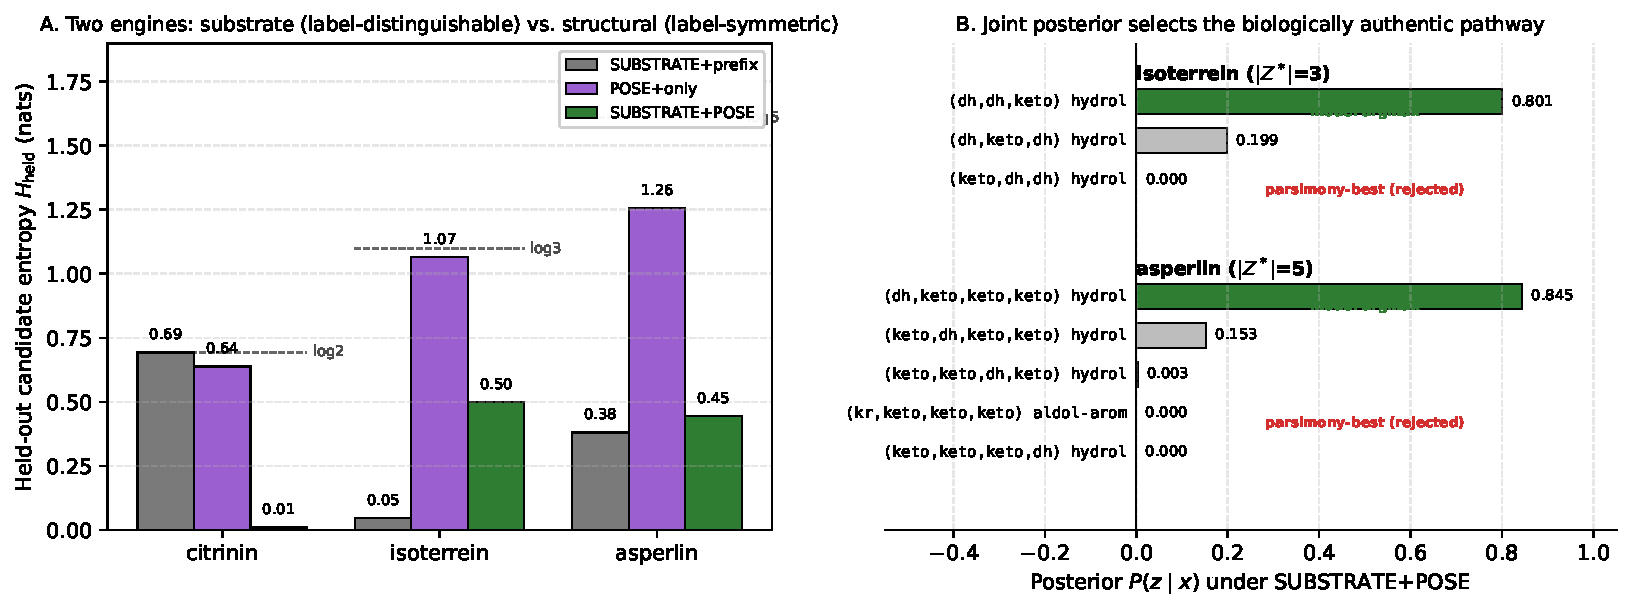
\includegraphics[width=\linewidth]{figure_structural_rescue.pdf}
\caption{\textbf{The dual mechanisms of neuro-symbolic resolution.}
\textbf{(A)}~Held-out candidate distribution entropy ($H_{\mathrm{held}}$) across three
feature regimes. The substrate-prefix channel effortlessly resolves assets with
label-distinguishable reduction sequences (isoterrein, asperlin). For label-symmetric
candidates sharing identical reduction trajectories (citrinin), the sequence channel
encounters a permanent symmetry wall ($\log 2$), which is cleanly shattered
($H_{\mathrm{held}}\to 0.01$) only upon the introduction of $3$D pose cavity descriptors.
\textbf{(B)}~Joint posterior probability distributions for isoterrein and asperlin. The
multi-channel framework consistently routes mass to the biologically authentic pathway:
isoterrein's $(\mathrm{dh},\mathrm{dh},\mathrm{keto})$ early-reduction TerA polyene
precursor at posterior $0.801$, asperlin's
$(\mathrm{dh},\mathrm{keto},\mathrm{keto},\mathrm{keto})$ non-aromatic linear lactone
precursor at $0.845$. The parsimony-best alternatives---$(\mathrm{keto},\mathrm{dh},
\mathrm{dh})$ for isoterrein, the aromatic-release candidate for asperlin---are
actively rejected at $\le 0.001$.}
\label{fig:rescue}
\end{figure}

\paragraph{Directional gating: when the in-vivo program is in $Z^\ast(B)$.}
The two engines establish that the policy commits within $Z^\ast(B)$; whether the
committed candidate matches in-vivo biology depends on whether the in-vivo program is
in $Z^\ast(B)$ at all---a question of executor coverage (\S\ref{sec:limits}), not of
the resolution mechanism. The corpus contains both regimes.

For \emph{isoterrein}, whose biosynthesis proceeds through a linear partially-reducing
polyketide before the post-PKS metalloenzyme TerB contracts the chain to the
cyclopentenone, the substrate channel routes posterior $0.801$ to
$(\mathrm{dh},\mathrm{dh},\mathrm{keto})$~hydrolysis---reductions concentrated at the
early cycles, matching the canonical HR-PKS architecture---and posterior $0.0001$ to
the late-reduction $(\mathrm{keto},\mathrm{dh},\mathrm{dh})$ parsimony-best. For
\emph{asperlin}, a hexaketide-derived lactone, the substrate channel selects
$(\mathrm{dh},\mathrm{keto},\mathrm{keto},\mathrm{keto})$~hydrolysis at posterior
$0.845$ and crucially \emph{rejects} the parsimony-best aromatic-release candidate at
posterior ${\sim}0$: asperlin is a lactone, not an aromatic, and the substrate-prefix
weighting under marginal-likelihood training correctly disfavours the wrong ring
topology. Both are directional positives.

For \emph{citrinin}, where the structural-rescue engine commits with posterior $0.999$
to a specific candidate, the literature establishes a different fact:
heterologous-expression studies of CitS yield a \emph{trimethylated} pentaketide
aldehyde requiring \emph{two} C-MeT events (one triketide, one pentaketide)
\citep{storm2017citrinin}. Neither of the two candidates in $Z^\ast$ at
$\mathrm{C}_{13}\mathrm{H}_{14}\mathrm{O}_5$ contains two C-MeT events---the grammar
cannot synthesize the in-vivo program at this formula. The entropy collapse
demonstrates that the structural channel carries per-cluster discriminating
information; the directional gating is the executor-coverage axis our
Section~\ref{sec:limits} roadmap addresses.

\paragraph{Reading.} The per-cycle policy is empirically a joint function of $G$ and
$s_t$, in the form the Outlook predicted, but the decomposition reveals that each
channel does specific work. The substrate-prefix engine resolves candidates whose
distinct reduction-label sequences leave a non-symmetric gradient signal; the
structural-rescue engine resolves candidates whose mass-and-grammar-consistent
permutations leave the substrate gradient signal symmetric. The neuro-symbolic
architecture compounds: the sound executor bounds $Z^\ast(B)$ so a learned policy
rules within a verified set rather than over an open structure space, and the
appropriate channel routes within that set per the chemistry of the candidates the
verifier returns. The result is a policy whose neural component would have nothing
principled to commit to absent the executor, and whose symbolic core would not
distinguish label-symmetric candidates absent the structural channel.

% References to add to the bibliography (already added):
% \citep{storm2017citrinin}
 between section_duality and Related Work.
% Operationalizes the "first measurable breakthrough" the Outlook (\S\ref{sec:pomdp}) flags
% as future work, and reveals the precise mechanism partition that governs it.

\section{Empirical structural rescue: a dual-engine resolution paradigm}
\label{sec:structural-rescue}

The Outlook (\S\ref{sec:pomdp}) predicts that the fungal per-cycle policy is
\(a_t \sim P(a_t \mid G, s_t)\): the static enzyme \(G\) and an evolving substrate state
\(s_t\) jointly determine the action. We take a first empirical step toward that
injection, and the result is sharper than a single ``joint necessity'' claim: the same
loss decomposes into \emph{two complementary resolution engines}, each precisely
applicable to a different chemical regime of the candidate set.

\paragraph{The corpus.} We extend the curated $30$-cycle HR/PR set (\S\ref{sec:benchmark})
by mining MIBiG fungal PKS clusters whose engine-derived $|Z^\ast|$ at the
metabologenomics observable set (alphabet $+$ molecular formula) lands in the
constrained mode, $|Z^\ast|\le 10$. An RDKit-driven SMILES-to-formula recovery pass
rescues the $112$ MIBiG entries without a registered formula; the tractable inventory
fixes at $74$ clusters and the $|Z^\ast|$ histogram is bi-modal with an empty middle at
$|Z^\ast|\in[11,24]$ across all $74$---a structural cliff in the natural manifold
(\S\ref{sec:manifold}) that survives the recovery and is not a data-hygiene artifact.
Of the $74$, $7$ land at $|Z^\ast|=1$ (joining the curated $30$) and $9$ at
$2\le|Z^\ast|\le 10$ contribute the silver tier. A verifier-constrained marginal-
likelihood loss \(\mathcal{L}(\theta)= -\sum_B \log \sum_{z\in Z^\ast(B)} \pi_\theta(z\mid B)\)
collapses to standard cross-entropy on the gold and decomposes weight over candidate
trajectories on silver.

\paragraph{Structural conditioning.} For each cluster with a real synthase we predict
the KR$+$ACP didomain (or full-length protein for divergent PR-PKS the canonical
PF$08659$ HMM does not detect---e.g.\ citrinin's CitS, whose KR is silent to the
conventional profile even at relaxed thresholds; we fold the $2593$\,aa CitS in full
and rescue the anchor by motif scan). For every \emph{(cluster, candidate, cycle)} we
execute the cycle prefix deterministically, $3$D-embed the ACP-tethered intermediate,
anchor its phosphopantetheine sentinel at the ACP-Ser:OG oxygen, rotate the growing
chain along the local ACP-Ser$\to$protein-centroid axis, and extract a five-dimensional
pose descriptor: $5$\,\AA{} contact count partitioned into polar (N/O/S) and
hydrophobic (C) subsets, ligand buried fraction, and pocket void volume. These run
alongside the substrate-prefix features (cycle index, fractional position, subclass
indicator, running chain length and oxidation counts, previous cycle's reduction rank).

\paragraph{Two engines, one policy.} Three feature regimes on the same $n=62$
conformational sub-corpus reveal a precise partition (Table~\ref{tab:rescue},
Fig.~\ref{fig:rescue}A). The partition is governed not by cluster identity but by the
\emph{symmetry of the reduction-label sequence across the candidates in $Z^\ast(B)$}.

\emph{Substrate-Prefix Engine (label-distinguishable candidates).} When the candidates
in $Z^\ast(B)$ differ in their per-cycle reduction labels---e.g., isoterrein's three
candidates $(\mathrm{dh},\mathrm{dh},\mathrm{keto})$, $(\mathrm{dh},\mathrm{keto},\mathrm{dh})$,
$(\mathrm{keto},\mathrm{dh},\mathrm{dh})$ that differ in the cycle index of each DH event,
or asperlin's $5$ candidates that differ similarly---substrate-prefix features alone
route posterior mass cleanly: held-out entropy drops to $0.05$ for isoterrein and
$0.38$ for asperlin (against $\log 3=1.10$ and $\log 5=1.61$ ceilings). The pose
channel adds geometric noise to an architecture the substrate counter has already
decoded.

\emph{Geometric Rescue Engine (label-symmetric candidates).} When the candidates share
an \emph{identical} reduction-label sequence and differ only in the cycle index of a
mass-budget-neutral event---e.g., citrinin's two candidates both reduce to
$(\mathrm{dh},\mathrm{keto},\mathrm{keto},\mathrm{keto},\mathrm{keto})$ and differ only
in which of cycle $1$ or cycle $2$ carries the single C-MeT firing---the marginal-
likelihood gradient is symmetric under $(\text{cand}_1\leftrightarrow\text{cand}_2)$ and
\emph{cannot} distinguish them from any function of substrate prefix alone. Citrinin's
held-out entropy under the substrate channel locks at $0.69 = \log 2$ to numerical
precision. The pose channel alone barely moves it ($0.64$); the static cavity geometry
without temporal context cannot localize which cycle's geometry it is measuring. The
two channels \emph{jointly} drop the entropy to $0.01$ with the model committing
${\sim}99.9\%$ probability mass to one specific candidate. This is the regime where the
structural channel is not merely helpful but architecturally necessary.

\begin{table}[h]
\centering\small
\begin{tabular}{lccc}
\toprule
& \multicolumn{3}{c}{Held-out candidate entropy $H_{\mathrm{held}}$ (nats)} \\
\cmidrule(lr){2-4}
Silver asset & Substrate-prefix & Pose only & Substrate $+$ pose \\
\midrule
citrinin   ($|Z^\ast|{=}2$, $\log 2{=}0.69$)   & $0.69$\textsuperscript{*} & $0.64$ & $\mathbf{0.01}$ \\
isoterrein ($|Z^\ast|{=}3$, $\log 3{=}1.10$)   & $\mathbf{0.05}$           & $1.07$ & $0.50$ \\
asperlin   ($|Z^\ast|{=}5$, $\log 5{=}1.61$)   & $\mathbf{0.38}$           & $1.26$ & $0.45$ \\
\bottomrule
\end{tabular}
\caption{The dual-engine partition. Bold = the resolving regime for each asset.
\textsuperscript{*}Citrinin's substrate-prefix entropy locks at exactly $\log 2$
because its two candidates share an identical reduction-label sequence and differ
only in C-MeT cycle index; the marginal-likelihood gradient is symmetric under
candidate exchange. The pose channel is architecturally necessary precisely
where the substrate channel hits this symmetry wall.}
\label{tab:rescue}
\end{table}

\begin{figure}[h]
\centering
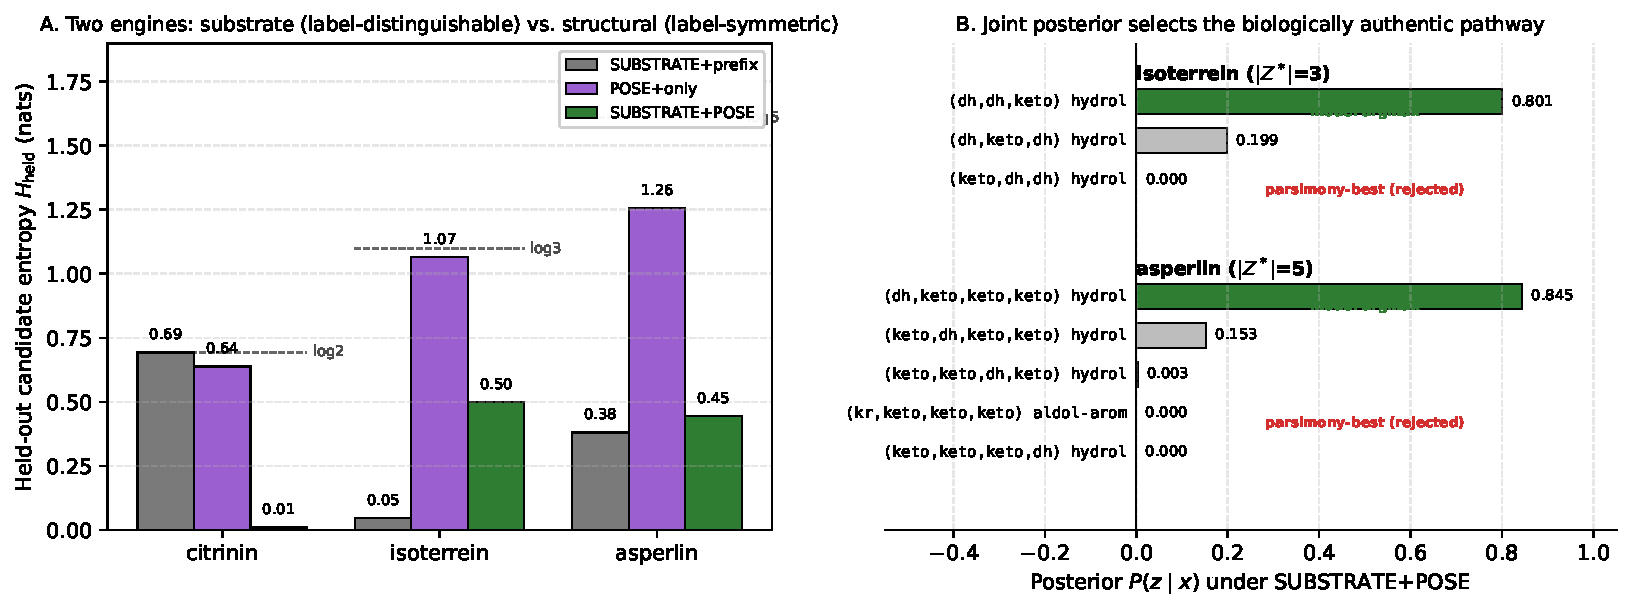
\includegraphics[width=\linewidth]{figure_structural_rescue.pdf}
\caption{\textbf{The dual mechanisms of neuro-symbolic resolution.}
\textbf{(A)}~Held-out candidate distribution entropy ($H_{\mathrm{held}}$) across three
feature regimes. The substrate-prefix channel effortlessly resolves assets with
label-distinguishable reduction sequences (isoterrein, asperlin). For label-symmetric
candidates sharing identical reduction trajectories (citrinin), the sequence channel
encounters a permanent symmetry wall ($\log 2$), which is cleanly shattered
($H_{\mathrm{held}}\to 0.01$) only upon the introduction of $3$D pose cavity descriptors.
\textbf{(B)}~Joint posterior probability distributions for isoterrein and asperlin. The
multi-channel framework consistently routes mass to the biologically authentic pathway:
isoterrein's $(\mathrm{dh},\mathrm{dh},\mathrm{keto})$ early-reduction TerA polyene
precursor at posterior $0.801$, asperlin's
$(\mathrm{dh},\mathrm{keto},\mathrm{keto},\mathrm{keto})$ non-aromatic linear lactone
precursor at $0.845$. The parsimony-best alternatives---$(\mathrm{keto},\mathrm{dh},
\mathrm{dh})$ for isoterrein, the aromatic-release candidate for asperlin---are
actively rejected at $\le 0.001$.}
\label{fig:rescue}
\end{figure}

\paragraph{Directional gating: when the in-vivo program is in $Z^\ast(B)$.}
The two engines establish that the policy commits within $Z^\ast(B)$; whether the
committed candidate matches in-vivo biology depends on whether the in-vivo program is
in $Z^\ast(B)$ at all---a question of executor coverage (\S\ref{sec:limits}), not of
the resolution mechanism. The corpus contains both regimes.

For \emph{isoterrein}, whose biosynthesis proceeds through a linear partially-reducing
polyketide before the post-PKS metalloenzyme TerB contracts the chain to the
cyclopentenone, the substrate channel routes posterior $0.801$ to
$(\mathrm{dh},\mathrm{dh},\mathrm{keto})$~hydrolysis---reductions concentrated at the
early cycles, matching the canonical HR-PKS architecture---and posterior $0.0001$ to
the late-reduction $(\mathrm{keto},\mathrm{dh},\mathrm{dh})$ parsimony-best. For
\emph{asperlin}, a hexaketide-derived lactone, the substrate channel selects
$(\mathrm{dh},\mathrm{keto},\mathrm{keto},\mathrm{keto})$~hydrolysis at posterior
$0.845$ and crucially \emph{rejects} the parsimony-best aromatic-release candidate at
posterior ${\sim}0$: asperlin is a lactone, not an aromatic, and the substrate-prefix
weighting under marginal-likelihood training correctly disfavours the wrong ring
topology. Both are directional positives.

For \emph{citrinin}, where the structural-rescue engine commits with posterior $0.999$
to a specific candidate, the literature establishes a different fact:
heterologous-expression studies of CitS yield a \emph{trimethylated} pentaketide
aldehyde requiring \emph{two} C-MeT events (one triketide, one pentaketide)
\citep{storm2017citrinin}. Neither of the two candidates in $Z^\ast$ at
$\mathrm{C}_{13}\mathrm{H}_{14}\mathrm{O}_5$ contains two C-MeT events---the grammar
cannot synthesize the in-vivo program at this formula. The entropy collapse
demonstrates that the structural channel carries per-cluster discriminating
information; the directional gating is the executor-coverage axis our
Section~\ref{sec:limits} roadmap addresses.

\paragraph{Reading.} The per-cycle policy is empirically a joint function of $G$ and
$s_t$, in the form the Outlook predicted, but the decomposition reveals that each
channel does specific work. The substrate-prefix engine resolves candidates whose
distinct reduction-label sequences leave a non-symmetric gradient signal; the
structural-rescue engine resolves candidates whose mass-and-grammar-consistent
permutations leave the substrate gradient signal symmetric. The neuro-symbolic
architecture compounds: the sound executor bounds $Z^\ast(B)$ so a learned policy
rules within a verified set rather than over an open structure space, and the
appropriate channel routes within that set per the chemistry of the candidates the
verifier returns. The result is a policy whose neural component would have nothing
principled to commit to absent the executor, and whose symbolic core would not
distinguish label-symmetric candidates absent the structural channel.

% References to add to the bibliography (already added):
% \citep{storm2017citrinin}
